\chapter{Background}
\label{background}

\section{Glycosaminoglycans (GAGs)}
\label{background:gags}


\subsubsection{Genral aspects}%The nature of GAGs}
Carbohydrates are ubiquitous building blocks found in all forms of life. As
implicated by their name, they are made of carbon, hydrogen and oxygen. Despite
this rather small set of atom types, an enormous variety of carbohydrates
exists. The origin of major parts of this diversity is of combinatorial nature:
carbohydrates usually occur as polysaccharides made of many connected
monosaccharides (or \enquote{sugar rings}), whereas various different types of
monosaccharides are available in nature. They are distinguishable by their
chemical configuration, and usually there are two stereoisomers for each of
those configurations, leading to a broad spectrum of different sugar rings whose
nomenclature and chemistry are described in detail in reference books
\cite{carbohydrate_chemistry_robyt_1998, carbohydrate_chemistry_royal_2000}.
Glycosaminoglycans (GAGs), reviewed in
\cite{essentials_glycobiology_gags_chapter_2009}, are a special class of
carbohydrates. GAGs play a critical role in many biological processes; they are
important for cell adhesion and cell growth, and their multifarious biological
activity arises from their ability to interact with and regulate a large number
of proteins \cite{handel_2005,gandhi_structure_2008}. GAGs are unbranched
(linear) saccharide chains, comprised of a periodically repeating unit, whereas
each unit is made of two pyranose (a six-membered ring consisting of five carbon
atoms and one oxygen atom) monosaccharides:

\nomenclature{GAG}{glycosaminoglycan}

\begin{itemize}
\item One is an amino sugar or \enquote{hexosamine}, either a
D\-/N\-/acetylglucosamine (GlcN) or a D\-/N\-/acetylgalactosamine (GalN).
\item The other is a uronic saccharide or \enquote{hexuronic acid}, either a
D-glucuronic acid (GlcA) or its C5\-/epimer L\-/iduronic acid (IdoA), or, in
seldom cases, a D\-/galactose (Gal).
\end{itemize}


\nomenclature{IdoA}{L-iduronic acid}
\nomenclature{GlcA}{D-glucuronic acid}
\nomenclature{GalN}{D-N-acetylgalactosamine}
\nomenclature{GlcN}{D-N-acetylglucosamine}


\begin{table}
\scriptsize
\centering
\renewcommand{\arraystretch}{1.3}
\begin{tabular}{lll}
\midrule
GAG type & main disaccharide & charge/\si{\elementarycharge} \\
\midrule
Heparin (HP) & L-IdoA2S-$\alpha$(1$\rightarrow$4)-D-GlcNS6S-$\alpha$(1$\rightarrow$4) & -4 \\
Chondroitin-4-sulfate (CS4) & D-GlcA-$\beta$(1$\rightarrow$3)-D-GalN4S-$\beta$(1$\rightarrow$4) & -2 \\
Hyaluronan (HA) & D-GlcA-$\beta$(1$\rightarrow$4)-D-GlcN-$\alpha$(1$\rightarrow$4) & -1 \\
\midrule
\end{tabular}
\caption{
Fundamentally different GAG types, their repeating disaccharide unit in IUPAC
nomenclature, and their charge per disaccharide, in units of the elementary
charge. The abbreviations given in brackets in column one are used throughout
this thesis.}
\label{tab:bg:gagtypes}
\end{table}

\nomenclature{HP}{heparin}
\nomenclature{HA}{hyaluronan}
\nomenclature{CS4}{chondroitin-4-sulfate}
\nomenclature{CS6}{chondroitin-4-sulfate}

A special feature of GAGs is that they are usually sulfated at various ring
positions, leading to a number of possible sulfation patterns per repeating
disaccharide unit. The number of possible combinations of basic disaccharide
units, two different allowed geometries of the glycosidic linkage between them,
and variations in the sulfation pattern imply that the heterogeneity among GAGs
is large. Still, physiologically occurring GAGs can be roughly categorized into
six major GAG types. Three of those, the most important ones for this thesis,
are listed in \cref{tab:bg:gagtypes} together with their repeating disaccharide
unit, sulfation pattern, glycosidic linkage type, and with their abbreviation
used here from now on. Three other major GAG types are usually listed in
literature \cite{gandhi_structure_2008}, which play a less important role in
this thesis than the ones listed in \cref{tab:bg:gagtypes}:

\begin{itemize}
\item Heparan sulfate, which is very similar to heparin, but with --- on average
--- a higher content of glucuronic acid than iduronic acid.
\item Dermatan sulfate, which is similar to chondroitin sulfate, but is built of
iduronic acid instead of glucuronic acid.
\item Keratan sulfate, the only GAG type that contains a D\-/galactose
saccharide instead of an acid. The amino sugar is the same as in chondroitin
sulfate.
\end{itemize}

Except for HA, which is the only non-sulfated GAG, the naturally occurring
sulfation of GAGs is strong, with up to three sulfate groups per disaccharide
unit in case of heparin. Considering the carboxyl group contained in the
hexuronic acid, each repeating disaccharide unit always carries at least one
negative charge at physiological pH (which is also true for HA). Adding
sulfation, this charge may grow up to -4 for heparin (see
\cref{tab:bg:gagtypes}), which in fact is the biological macromolecule with the
largest charge density known \cite{capila_linhardt_hep_prot_2002}.
\Cref{fig:bg:heparin_chemstruct} shows the chemical configuration of the
repeating disaccharide unit of heparin and schematically visualizes its
structure in space. What is depicted there actually is the disaccharide unit
which occurs \textit{most frequently} in natural heparin polysaccharides.
Polymeric GAGs in an organism can be quite long with a molecular weight of about
10 to 100\,kDa \cite{gandhi_structure_2008}, and they never reach
\SI{100}{\percent} purity. That is, natural GAGs are always comprised of a
mixture of more than only two monosaccharides, and the repeating units shown in
\cref{tab:bg:gagtypes} are the \textit{dominating} ones for each of the cases.

\begin{figure}
\centering
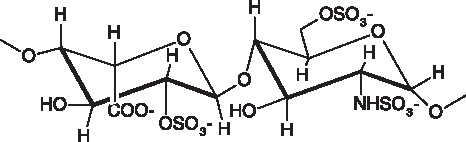
\includegraphics[width=1.0\textwidth]{gfx/background/hp_repeating_unit_structure_01.pdf}
\caption[]{
Molecular configuration of the repeating disaccharide unit of heparin (the one
which occurs most frequently in natural heparin polysaccharides). The pyranose
to the left is a 2-O-sulfated iduronic acid (IdoA2S), connected via a
1$\rightarrow$4 glycosidic linkage to the 6-O-sulfated
2-deoxy-2-sulfamido-α-D-N\-/acetylglucosamine (GlcNS6S). At physiological pH,
the charge of this disaccharide is -4 elementary charges.
}
\label{fig:bg:heparin_chemstruct}
\end{figure}

There are many more than six GAG variants with established names, such as
Chondroitin\-/6\-/sulfate (CS6), which is the same as CS4, but sulfated at the
C6 position of the galactosamine instead of in the fourth position. With the GAG
types described here so far, all major characteristics of naturally occurring
GAG molecules are covered. Other GAG types are not listed, because they are not
fundamentally different from what has been described and therefore were not
investigated in the framework of this thesis.

In organisms, all GAG chains except for HA  appear covalently bound to a core
protein, comprising a so-called \textit{proteoglycan} complex
\cite{essentials_glycobiology_gags_chapter_2009}. These large structures consist
of a linear protein with many GAGs covalently linked to it. Each GAG is linked
to the core protein via a special sugar linker, which itself is attached to
(usually) a serine residue of the core protein. As of the length of the GAG
chains, however, the biological functions of proteoglycans depend to a large
extent only on the interaction of its GAG chain(s) with other proteins, i.e.\
the free end of a GAG chain can be considered unaffected by the core protein.
This is one of the fundamental assumptions applied in this thesis project: GAGs
are treated as \textit{free} molecules.



%While it is likely
%that their tremendous length and also their covalent linkage to proteoglycans
%serve have an overall impact on the biological function of GAGs, it is a
%valid and well-established approximation to not account for these facts in
%molecular modeling studies that aim for resolving the molecular mechanism of
%protein-GAG interaction in atomic detail... in a biological function and overall  treated as






\subsubsection{Monosaccharide conformations}

The origin and geometry of various pyranose monosaccharide conformations is
comprehesibly classified and discussed in
\cite{classification_pyranose_conformers_1960}. The conformational nomenclature
used throughout this thesis follows IUPAC rules, which are well-described in
\cite{iupac_gag_conformations_1980}.

Most monosaccharide rings in GAGs have a predominant ring conformation, and can
be considered rigid, as is the case for e.g.\ N-acetyl-D-glucosamine (GlcN),
which mainly exists as ${}^{4}\mathrm{C}_1$ chair, which becomes especially
stable when the GlcN becomes sulfated \cite{Sattelle_glcnac_right_chair_2011},
as in heparin.


\subsubsection{General aspects about protein-GAG interaction}

are play a critical role in many biological processes.
Their multifarious biological activity arises from their ability to interact
with and regulate a large number of proteins.

% All the rest is from \cite{essentials_glycobiology_protgags_2009}
More than 100 glycosaminoglycan (GAG)-binding proteins have been described in the literature, falling into the broad classes presented in Table 35.1. To a large extent, these studies have focused on protein interactions with heparin, which is a more highly sulfated, iduronic acid (IdoA)-rich form of heparan sulfate (HS; Chapter 16). This bias may reflect the commercial availability of heparin, which is frequently used for fractionation studies and heparin-Sepharose affinity chromatography. The binding of protein ligands to heparin is thought to mimic the physiological interaction of proteins with the HSs present on cell surfaces and in the extracellular matrix. In comparison, relatively few proteins are known to interact with chondroitin sulfate (CS) or keratan sulfate (KS) with comparable avidity and affinity. In some cases, CS and the related GAG dermatan sulfate (DS) may be physiologically relevant binding partners because these GAGs predominate in many tissues. Determining the physiological relevance of these interactions is a major area of research.



\subsubsection{Structure of GAGs}

show GAG oligosaccharide structure in space, quote mulloy et al regarding
oligosaccharide structure modeling from NMR etc.



\section{A primer on IL-10 biology}

 IL-10's biological function is mainly considered to be
, but

 has pleiotropic effects in immunoregulation and
inflammation.


        in closing remarks, relate to extracellular matrix


%\subsubsection{GAG structures used in \textit{in silico} experiments}


\section{IL-10 and its relation to GAGs}


 anti-inflammatory

- Relevance of IL-10 in immune regulation
- Bio-relevant IL-10-GAG interaction? Motivated by Salek ardakini.

We are interested in GAG interaction with the cytokine interleukin-10 (IL-10,
reviewed in \cite{moore_2001}), which is generally considered to exert an
immunosuppressive function. From \textit{in vitro} experiments, IL-10 is known
to bind GAGs and there is evidence that GAGs may modulate its biological
function \cite{salek_ardakani_2000}. So far however, no structural detail about
IL-10-GAG interaction is known.


Wherever IL-10 is supposed to
regulate an immune response, for instance in the process of wound healing and
tissue regeneration, GAGs are


\section{In-silico methods for investigating protein-GAG interaction}


\subsubsection{GAG representation approximations: length, purity}



A more severe approximation applied in this thesis is the treatment of GAGs as
\textit{short} molecules. Considering the  mostly ranging from tetra- to hexasaccharides. Considering the level of atomic detail aimed for ... to be observed... in this
thesis project, GAGs are modeled as short molecules.


Also, when treating GAGs as short molecules, they are represented by the ideal
periodic repetition of the most frequently observed disaccharide unit,
impurities or variations in the monosaccharide sequence are ignored.

ir ideal periodic

explain DP, degree of polymerization


\subsection{A primer on docking methods}


    - Methods applied in literature: a mini review
        AutoDock3 stands out, just by experience, not by concept
    - Problems of different complexity: local vs. global docking.
    - (AutoDock 3 protein-GAG blind docking validation study,
        Method, results, discussion, conclusion)

\lipsum[1-5]

\subsection{A primer on molecular dynamics simulations}

\lipsum[1-5]

\subsubsection{End-point free energy methods (\enquote{MM-PB(GB)SA})}
% This label is required in DMD chapter.
\label{methods:mmpbsa_mmgbsa}


Cite this: \cite{schlick_innovationsdynamics_2012} (volume 2, chapter 12).

\lipsum[1-5]

\section{Structure of IL-10 and its receptors}

    - Structure description
        exists mainly as homodimer [
            biochemistry, 1998, 37, 16943-16951, zdanov 1995]


    - IL-10 and its receptors
        - what is known in literature (current state of knowlege)
            R1+IL-10 structure
            R2 structure
            ternary complex binding models
            what is required for signaling? literature overview
        - a critical review: monomer
            minimal unit required for signaling (monomer)
        - IL-10 + R1 + R2 structure model from IL20 ternary complex


\section{Aim and scope of this thesis}

- Vision: gaining control over IL-10 function in artificial extracellular matrices

- Motivation and goal: investigate IL-10-GAG system with computational
      methods, in collaboration with...

The aim of this project is to unravel atomic details of IL-10-GAG interaction
with theoretical and computational means. If required, methodological approaches
are to be developed. Integration of \textit{in silico}-based predictions with
experimental results from collaborators will hopefully provide insights into the
mechanisms determining IL-10-GAG interaction. Methodology developed during this
project is applicable to protein-GAG systems in general, rendering it valuable
for a large field of research.



\hl{cite interleukin-2 -heparin interaction (mulloy, rider) !}

\lipsum[1-5]





